% -*- mode: latex; fill-column: 80; -*-
\documentclass[a4paper,10pt]{report}
\setcounter{secnumdepth}{3}

\hoffset=-0.75in
\voffset=-1in
\textwidth=450pt
\textheight=720pt

\usepackage{amsmath}
\usepackage[type={CC},modifier={by-sa},version={4.0}]{doclicense}
\usepackage{enumitem}
\usepackage{hyperref}
\hypersetup{
  colorlinks,
  citecolor=blue,
  filecolor=blue,
  linkcolor=blue,
  urlcolor=blue
}

\usepackage{graphicx}
\graphicspath{ {./image/} }

\usepackage{subcaption}
\usepackage{listings}

\def\FlintVersion{2.4}
\def\FlintLongVersion{2.4.0}
\def\Flint{Flint~\FlintVersion}
\def\Tagline{a simulator for biological and physiological models}
\def\FlintFilenamePrefix{Flint-\FlintLongVersion}

\newcommand{\filename}[1]{{\tt #1}}

\newcommand\FigureOfImage[2]{\begin{figure}[h]
  \centering
  \includegraphics[width=0.8\textwidth]{#1}
  \caption{#2}\label{fig:#1}
\end{figure}}

\title{\Flint: The User Guide}
\author{Flint project}

\makeindex

\begin{document}

\maketitle

\begin{abstract}
This document describes how to use \Flint, \Tagline.
Readers also find some platform-specific notes and trouble-shooting techniques that
users would like to know when using \Flint.
\end{abstract}

\tableofcontents

\vfill

\doclicenseThis

%%%%%%%%%%%%%%%%%%%%%%%%%%%%%%%%%%%%%%%%%%%%%%%%%%%%%%%%%%%%%%%%%%%%%%%%

\chapter{Introduction}

Understanding dynamics of living organisms often requires a mathematical model
that describes the hypotheses to be tested. It is widely recognized that the
class of ordinary differential equations (ODE) is suitable for describing the
time course of variables in a deterministic system, stemming from a simple
assumption about the rate of their change.
One of such examples is the chemical reaction accelerated by an enzyme
following the Michaelis-Menten kinetics; another is the action potential of
cardiac cells driven by modulation of ion channels. By a virtue of
differential equations, these celullar models can be integrated into the one of
tissue or organ level. In fact, the way to integrate a computational model of
the physiological functions of the whole individual has been explored since the
end of the last century, under the name physiome \cite{leem_perspectives_2016}.

It is, however, technically challenging for practitioners in the field of
biology or physiology to express their hypotheses on biological organisms in a
precise system of ODEs. In order to make it easier to edit a model in problem
that implicitly specify the ODEs, several domain-specific languages have
been proposed and standardized, including CellML \cite{CellML}, the
Physiological Hierarchy Markup Language (PHML) reported by
\cite{PHML}, and the Systems Biology Markup Language (SBML) reported
by \cite{SBML}. Although the design principle of each modeling
language varies, computational analysis of any model in these languages
comprises the shared set of procedures based on the theory of differential
equations and dynamical systems.

Flint is a simulator software for models written in the above languages, and
aims to provide an open, language-agnostic resource for reproducible simulation
studies. The simulator allows users to transform a given model into a system of
ODEs and solve it in a numerical manner. It also supports stochastic
differential equations (SDE), a non-deterministic extension of ODEs, which makes
it possible to involve random elements, e.g. noises, in the dynamics.

\section{Brief summary about \Flint}
\Flint~is new implementation of Flint 1.x, \Tagline.
Flint can run simulations of multi-level physiological models written in PHML.
It means that Flint parses given models, performs numerical analysis for their
simulation, and renders simulation outcome into a line graph via gnuplot \cite{gnuplot}.
Likewise, Flint can handle CellML and SBML as well as SBML-PHML hybrid models.

\subsection{Markup languages}
\Flint\ supports the following standard languages of models:
\begin{itemize}
\item PHML (including its precursor ISML \cite{ISML})
\item SBML
\item CellML
\end{itemize}

\subsection{Available numerical algorithms for ordinary differential equations}
\Flint\ supports the following algorithms to solve ODEs numerically:
\begin{itemize}
\item Euler method
\item Runge-Kutta 4th-order method
\item Adaptive stepsize Runge-Kutta method, based on the ARKode solver of
  SUNDIALS \cite{hindmarsh2005sundials}
\end{itemize}

\subsection{Available numerical algorithms for stochastic differential equations}
\Flint\ also supports the following algorithms to solve SDEs
numerically:
\begin{itemize}
\item Euler-Maruyama method \cite{Allen2007}
\end{itemize}

\section{Notation}
In this document, a sentence starting with {\tt \$} describes a command line in
a command shell on your system, such as\\
{\tt \$ echo this is a command line.}


%%%%%%%%%%%%%%%%%%%%%%%%%%%%%%%%%%%%%%%%%%%%%%%%%%%%%%%%%%%%%%%%%%%%%%%%

\chapter{Getting started}

This chapter explains how to obtain and install Flint, and describes how to run
a simulation.

\section{Supported platforms}
\Flint\ runs on several supported platforms, including:
\begin{itemize}
\item Windows 7 or later;
\item macOS: OS X El Captian (10.11) or later;
\item Linux distributions such as Debian 10, Ubuntu 18.04, and RHEL/CentOS 7 or 8.
\end{itemize}

\section{Download and install \Flint}
Flint project distributes \Flint's x86-64 binary installers for Windows,
macOS, and CentOS/RHEL 7 or 8.

\subsection{On Windows}
Please download the installer package
\filename{\FlintFilenamePrefix-windows.x86\_64.msi} at
\url{https://sourceforge.net/projects/flintproject/files/Flint/}.
Double-clicking the .msi package will start the installation process.
If installed successfully, Flint's executable program will be found at\\
\filename{C:\textbackslash Program Files\textbackslash Flint\textbackslash flint.exe}.

\subsection{On macOS}
Please download the installer package \filename{\FlintFilenamePrefix-mac.dmg} at
\url{https://sourceforge.net/projects/flintproject/files/Flint/}.
The .dmg archive for macOS contains \Flint's .pkg file; extracting and
double-clicking it to start an application bundle called\\
\filename{Flint.app}.

\subsection{On CentOS/RHEL}
Please download \filename{\FlintFilenamePrefix-el7.x86\_64.zip} or
\filename{\FlintFilenamePrefix-el8.x86\_64.zip}
at \url{https://sourceforge.net/projects/flintproject/files/Flint/}, depending
on the major version of your OS.
Unzipping the archive, run the following command on a bash-like shell to install
RPM packages in it:
\begin{verbatim}
$ unzip Flint-*-el*.x86_64.zip
$ cd Flint-*-el*.x86_64
$ sudo rpm -Uvh --replacepkgs flint-*.rpm
\end{verbatim}
Once installed, Flint's executable will be found at\\
\filename{/opt/flint/bin/flint}.

\subsection{On other supported OSes}
In principle \Flint\ runs on any Linux distribution coming up with GTK 2 or 3.
You can build Flint from its source tarball, available at
\url{https://github.com/flintproject/Flint/archive/\FlintFilenamePrefix.tar.gz},
by following the instructions in \filename{INSTALL.org} found in the archive.

\section{Try your first simulation with \Flint}
This section describes a simple procedure with \Flint\ to run a simulation of an
example PHML model, which replicates the system of ordinary differential
equations about membrane potentials in nerve introduced by
\cite{hodgkin_quantitative_1952}.
If you have installed \Flint\ via one of its binary installer packages, the
model file can be found at\\
\filename{C:\textbackslash Program Files\textbackslash Flint\textbackslash  flint.exe}
on Windows,\\
\filename{Flint.app/Contents/Resources/example/HodgkinHuxley\_1952\_neuron\_model.phml}
on macOS, or\\
\filename{/opt/flint/example/HodgkinHuxley\_1952\_neuron\_model.phml} on CentOS/RHEL.\\
Otherwise you can also download it from\\
\url{https://github.com/flintproject/Flint/tree/\FlintFilenamePrefix/example/HodgkinHuxley\_1952\_neuron\_model.phml}.

\begin{description}
\item[Launch Flint] \hfill \\
To launch Flint, double-click
\filename{C:\textbackslash Program Files\textbackslash Flint\textbackslash flint.exe} on Windows,\\
\filename{Flint.app} on macOS, or \filename{/opt/flint/bin/flint} on CentOS/RHEL.\\
It shows a window like Fig.~\ref{fig:initial}.
\FigureOfImage{initial}{The initial window of Flint.}

\item[Open a model] \hfill \\
In the ``File'' menu, select ``Open'' to choose a model file. Then you will see
a file dialog like Fig.~\ref{fig:open-model}.
\FigureOfImage{open-model}{The file dialog to open a model.}
Select \filename{HodgkinHuxley\_1952\_neuron\_model.phml} in the file dialog
\footnote{On macOS, opening a form by {\tt Command}+{\tt Shift}+{\tt g}, one can
specify an absolute path in the application bundle \filename{Flint.app}.},
and click ``Open'' button.
Then the model window will appear as in Fig.~\ref{fig:hh}.
\FigureOfImage{hh}{The model window.}

\item[Choose duration and time step] \hfill \\
Specify the duration of simulation in ``Simulation Length'' and the time step
length of the simulation in ``Simulation Time Step'' optionally.

\item[Run a simulation] \hfill \\
Click the ``Run'' button to start a simulation.

Once simulation started running, the progress bar will appear in the control
panel in the right side like Fig.~\ref{fig:hh-progress}, and both the cross mark
(as ``Cancel'') and ``Detail'' buttons will be enabled.
\FigureOfImage{hh-progress}{The progress bar for the model.}

Wait until the status bar tells that the simulation completed (see
Fig.~\ref{fig:hh-completed}).
\FigureOfImage{hh-completed}{The status bar indicates the simulation completed.}

\item[See detail of the simulation] \hfill \\
Click the ``Detail'' button to get the simulation result.
Then a detail window will appear as in Fig.~\ref{fig:hh-detail}.
\FigureOfImage{hh-detail}{The detail window.}

\item[Select ordinates] \hfill \\
Click the ``View'' button on the detail window, then a plot window to render
line graphs about the simulation result, like Fig.~\ref{fig:hh-plot}.
\FigureOfImage{hh-plot}{The plot window.}
Check the Y1 column of ``V'' in the variable list, which calls gnuplot.
Soon the corresponding line graph will appear on a separate window,
like Fig.~\ref{fig:hh-plot-v}.
\FigureOfImage{hh-plot-v}{The plot window with ``V'' on Y1.}
Moreover you can also check the Y2 column of another variable ``I\_Na'' in the
list to arrange two line graphs in the same canvas, as in
Fig.~\ref{fig:hh-plot-v-ina}.
\FigureOfImage{hh-plot-v-ina}{The plot window with ``V'' on Y1 and ``I\_Na''
on Y2.}
\end{description}


%%%%%%%%%%%%%%%%%%%%%%%%%%%%%%%%%%%%%%%%%%%%%%%%%%%%%%%%%%%%%%%%%%%%%%%%

\chapter{Graphical User Interface}
\Flint\ comes with a graphical user interface out of the box. This chapter
explains features of the GUI and how to use them.

\section{Launching Flint}
On Windows, double-clicking \filename{flint.exe} in the start menu starts Flint.
On macOS, double-clicking \filename{Flint.app} works similarly.

\section{Quitting Flint}
To quit Flint, use the menu ``File''$\rightarrow$``Exit''.

\section{Loading models}
Flint must load models before running simulations for them.
Users tell Flint which model should be loaded by opening the model file.
Loading a model can fail due to some reasons; for example, it may fail if
the model file contains an error or unsupported elements.
An error dialog will display a diagnosis message when loading a model fails.
Once loading a model successfully, the model window shows up and stays
in the main window until closed, like Fig.~\ref{fig:lr}.

\section{Configuring simulation tasks}
\FigureOfImage{lr}{The model window.}
Before starting simulations for a loaded model, users may want to configure them
in terms of numerical integration, simulation time, output data, and parameters.

\subsection{Integration method}
Users have to choose a solver method for ordinary differential equations or
stochastic differential equations at the ``Integration method'' combobox.
An error will occur at simulation time when choosing any method except
the Euler-Maruyama method for a model including SDEs.

\subsection{Simulation Length}
Users must specify the total length of simulation time at the ``Simulation Length''
field; the given number is interpreted in terms of the selected time unit.

\subsection{Simulation Time Step}
Similarly to ``Simulation Length'', users can specify the time step at the
``Simulation Time Step'' field.

\subsection{Starting from}
Users can specify when (in the sense of simulation time) output starts from
at this field. By default, simulation process produces output from time 0.

\subsection{Data Sampling}
This setting is for determining how often the result data are written in.
Note that the sampling rate does not affect the calculation for simulation.

\subsection{Select output variables}
Before starting simulations for a loaded model, users may want to choose a
limited number of variables for output among available variables.
Filtering output variables will reduce the burden of writing output, and thus
may improve the simulation performance.
The ``Output Variables'' panel (Fig.~\ref{fig:lr-output-variables}) allows
user to select output variables by matching one of their properties with a given
string. The possible target properties depend on the format of the model file,
and are summarized in Table~\ref{tab:outputproperties}. With the ``Filter Column''
combo box one can choose the target. The ``Filter Pattern'' combo box chooses
the way to interpret the given string: as a regular expression (default), or
just as a fixed string.
\FigureOfImage{lr-output-variables}{The ``Output Variables'' panel.}
\begin{table}
\centering
\caption{Output variable's properties to be matched} \label{tab:outputproperties}
\begin{tabular}{l|c}
  Model file format & properties \\
  \hline
  PHML & Physical-quantity name; Module name \\
  SBML & Species or reaction name \\
  CellML & Variable name; Component name \\
\end{tabular}
\end{table}

\subsection{Parameterize constant values}
By default, Flint runs a single simulation job for each loaded model.
It is also possible to start a simulation batch for each model with
different values of parameters.
A batch of simulations can result in multiple different trajectories of
variables in the same model. Hereafter, we simply call each result from
an element in the batch a trajectory.

In order to explain the feature to parameterize constants found in a model,
let's define some technical terms as follows.
In Flint's terminology, named numeric constants in the model are called
shortly ``constants''.
For example, some of CellML's \verb|variable|s have attribute
\verb|initial_value|, which is assigned to a constant number.
In PHML there is an element called \verb|static-parameter| specifying a constant,
as well as \verb|initial-value|.
SBML's \verb|parameter| element has attribute \verb|value| assigned to a number.
All of them are constants in Flint's context, and they are potential targets for
changing their values by some parameters.
However, make sure that a constant in the above sense is \emph{not} a parameter
itself in Flint.
Rather, a constant can be parameterized by zero or more parameters.

In Flint's terminology, a parameter is a named object assigned to a specific
number for each trajectory.
Let $\mathcal{P}$ be the set of parameters.
To configure a batch, every parameter is bound to its own set of possible
values, called value-set.
Let $\mathcal{V}(p)$ be the value-set of parameter $p$ in $\mathcal{P})$.
The whole set of possible tuples of multiple parameters is defined as the
Cartesian product of multiple value-sets, i.e., $\prod_{p \in \mathcal{P}}
\mathcal{V}(p)$.
(It is also possible to custom how to construct the whole set of value tuples
for an advanced setting. Please read \ref{subsubsec:productzip}.)
From now on, a pair $(\mathcal{P}, \mathcal{V})$ is called the parameter set as
it determines the parameterization of a batch completely.

Given the parameter set of a batch, Flint will run as many simulations for the
given model as the cardinality of the Cartesian product, i.e.,
$\lvert \prod_{p \in \mathcal{P}} \mathcal{V}(p) \rvert$, by changing the
assigned values from a tuple to another.
In other words, each trajectory corresponds to a value tuple of the parameters.

Users can see and modify numeric values of constants in a loaded model,
such as the initial values of ordinary differential equations and values of
\verb|static-parameter|s of PHML, at the ``Parameters'' panel.
The table at the ``Parameters'' consists of each row corresponding to a constant
element in the model; the ``Expression'' field of the row accepts an algebraic
formula defining the parameterized value of the constant.
The following~\ref{subsubsec:formula-operator} summarize available operators in
the formula, which semantics conforms to MathML 3 \cite{MathML} in principle,
except infix operators such as \verb|+|, \verb|*|, etc.
For example, given parameters \verb|p| and \verb|q|, you can build a formula
like ``\verb|2.5 * max(p, 1) - cos(q)|''.

\subsubsection{Available operators to build a formula}\label{subsubsec:formula-operator}

\begin{itemize}
\item \verb|+| (infix): addition
\item \verb|-| (infix): subtraction
\item \verb|*| (infix): multiplication
\item \verb|/| (infix): division
\item \verb|%| (infix): remainder
\item
  \verb|abs|,
  \verb|arccos|,
  \verb|arccosh|,
  \verb|arccot|,
  \verb|arccoth|,
  \verb|arccsc|,
  \verb|arccsch|,
  \verb|arcsec|,
  \verb|arcsech|,
  \verb|arcsin|,
  \verb|arcsinh|,
  \verb|arctan|,
  \verb|arctanh|,
  \verb|ceiling|,
  \verb|cos|,
  \verb|cosh|,
  \verb|cot|,
  \verb|coth|,
  \verb|csc|,
  \verb|csch|,
  \verb|exp|,
  \verb|floor|,
  \verb|ln|,
  \verb|log|,
  \verb|max|,
  \verb|min|,
  \verb|power|,
  \verb|root|,
  \verb|sec|,
  \verb|sech|,
  \verb|sin|,
  \verb|sinh|,
  \verb|tan|,
  \verb|tanh|
  : mathematical functions
\end{itemize}

\begin{figure}[h]
  \centering
  \begin{subfigure}[b]{0.45\textwidth}
    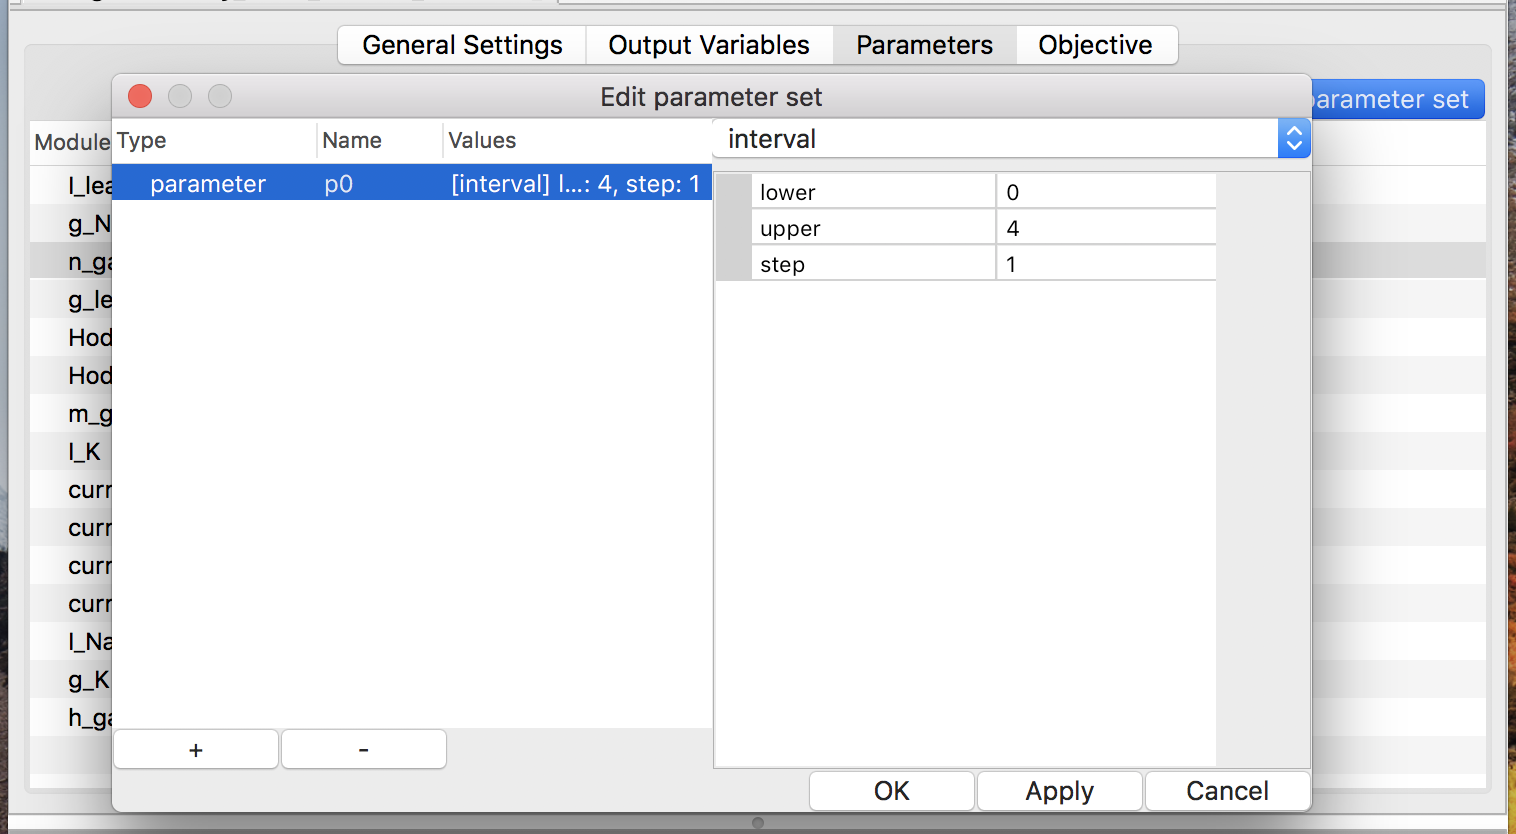
\includegraphics[width=\textwidth]{lr-edit-parameter-set-a}
    \caption{edit a parameter called ``p0''}\label{fig:lr-edit-parameter-set-a}
  \end{subfigure}
  \begin{subfigure}[b]{0.45\textwidth}
    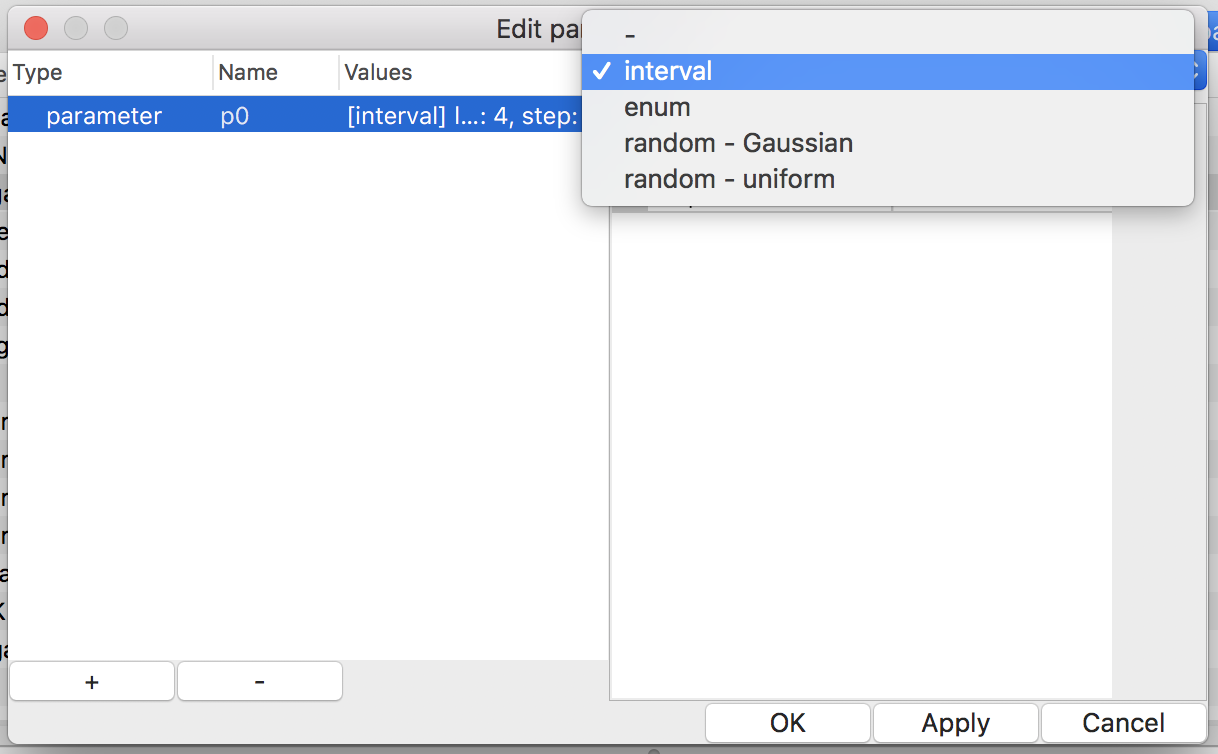
\includegraphics[width=\textwidth]{lr-edit-parameter-set-b}
    \caption{choosing value-set type}\label{fig:lr-edit-parameter-set-b}
  \end{subfigure}
  \caption{Editing the parameter set in the ``Edit parameter set'' window.}
\end{figure}

\subsubsection{Edit the parameter set}
In order to define or modify the parameter set, push button ``Edit parameter
set'' at first. Then a window will pop up. It allows users to see existing
parameters, add a new parameter (via the ``\verb|+|'' button), delete existing
one (via the ``\verb|-|'' button), and modify them (see
Fig.~\ref{fig:lr-edit-parameter-set-a}).

The name of a parameter is arbitrary, but must start with an alphabet or
underscore (\verb|_|), followed by a sequence of alphabets, underscores, and/or
digits (\verb|0|, \verb|1|, ..., \verb|9|).

There are four types of value-sets: enum, interval, Gaussian, and uniform
(see Fig.~\ref{fig:lr-edit-parameter-set-b}).
For a value-set of type enum, each of possible values must be specified.
On the other hand, only the lower and upper (both inclusive) of a range
of values with a step are required to define a value-set of type interval.
Note that possible values of an enum should be separated by a comma or a space.
The latter two types of value-sets are for generating pseudo-random values
according to specified probability distribution in simulation time.

\subsubsection{Define constants by parameters}
Once users have defined a parameter, it is available in the ``Expression'' field
of any row in the ``Parameters'' table (see Fig.~\ref{fig:lr-parameter-set}).
\FigureOfImage{lr-parameter-set}{Parameterize a constant with parameter ``p0''.}

\subsubsection{Control how to combine parameters}\label{subsubsec:productzip}
It will be often found that the whole set of possible tuples of the parameters
becomes too big even for the case of a small number of the parameters, i.e., that
$\lvert \mathcal{P} \rvert$ is small. For example, if you use five parameters
and each of them has a value-set of size 100, then the number of simulations
in the batch is $100^5$, which is more than $2^{33}$, so the run will never finish
within a realistic time frame.

To mitigate the explosion of the number of the combinations, there is a way
to skip some combinations; choose ``zip'' when creating an item by the
``\verb|+|'' button in the ``Edit parameter set'' dialog
(see Fig.~\ref{fig:lr-edit-parameter-set-productzip}).
Then, the value tuples of the parameters in the ``zip'' sub-tree are constructed
as like the \verb|zip()| function of the Python standard library
\cite{pythonstdlib} applies to their value-sets.
To be precise, let $\{p_1, p_2, ..., p_m\}$ be the parameters in the sub-tree,
and $n_i := \lvert \mathcal{V}(p_i) \rvert$.
The set of their value tuples is
\[
\left\{(v_{1 k}, v_{2 k}, ..., v_{m k}) \mid k = 1, 2, ..., n_i \right\},
\]
where the values in $\mathcal{V}(p_i)$ are ordered and enumerated as
$\{v_{i 1}, v_{i 2}, ..., v_{i n_i} \}$.
If $n_i$ varies, then the smallest $n_i$ is taken and the rest of values is
ignored.

For instance, suppose three parameters \verb|p|, \verb|q|, and \verb|r| belong
to a ``zip'' sub-tree. Let
\begin{align}
\mathcal{V}(p) &= \{0.1, 0.2, 0.3, 0.4, 0.5\};\nonumber\\
\mathcal{V}(q) &= \{3, 1, 4, 1, 5, 9\};\nonumber\\
\mathcal{V}(r) &= \{2, 3, 5, 7, 11, 13, 17\},\nonumber
\end{align}
where the elements of each value-set are ordered as shown.
Then the set of their value tuple is $\{(0.1, 3, 2), (0.2, 1, 3), (0.3, 4, 5),
(0.4, 1, 7), (0.5, 5, 11)\}$, which has only five elements.

The ``zip''-ped parameters can be combined with other parameters as by default,
i.e., by taking the Cartesian product; choose ``product'' when creating an
the ``\verb|+|'' button in the ``Edit parameter set'' dialog
(see Fig.~\ref{fig:lr-edit-parameter-set-productzip}).
Then, the items in the ``product'' sub-tree are combined by the Cartesian
product.
\FigureOfImage{lr-edit-parameter-set-productzip}{``zip'' and ``product'' in the ``Edit parameter set'' window.}

\section{Starting simulation}
To start simulation, use the menu ``Control''$\rightarrow$``Run'' or button
``Run'' on the control panel. It kicks simulation jobs for all loaded models.
Users can monitor the progress in total on the control panel, as well as the
one for a single job on the detail windows like Fig.~\ref{fig:lr-detail}.
Note that a context menu allows users to cancel simulation assigned to a
specific parameter value in a task.
\FigureOfImage{lr-detail}{The detail window during simulation.}

\section{Controlling simulation jobs}
After starting simulation jobs, users can control them instead of just waiting
for them finishing.

\subsection{Cancel jobs}
There is another way to cancel running jobs; pushing the cross mark on the
control panel (see Fig.~\ref{fig:lr-progress}), which cancels a job i.e. all
of its tasks together.
\FigureOfImage{lr-progress}{The progress bar / cross mark / ``Detail'' button on
 the control panel.}

\subsection{Pause and resume jobs}
As in Fig.~\ref{fig:control}, users can pause jobs at any time during simulation
by using the menu ``Control''$\rightarrow$``Pause''. Resuming paused jobs can
be done with the menu ``Control''$\rightarrow$``Resume''.
Note that this operation affects all of alive jobs simultaneously.
\FigureOfImage{control}{The Control Menu.}

\section{Visualizing simulation results}
Flint has a feature to show a line graph for the result of a simulation on the
fly, not only after its job finished, but also int the middle of ongoing
simulation.

From the detail window, users can display the plot window by clicking button
``View'' for each simulation job.

\subsection{Choose abscissa and ordinates}
In order to draw a line graph, users have to specify the abscissa and ordinates
by checking an X column as well as either Y1 or Y2 column.
Immediately after choosing abscissa and ordinates, Flint calls gnuplot in the
background to draw a line graph.
Thus users have to install gnuplot in advance, and to specify the location of
the gnuplot executable (see section~\ref{sec:preference}).

\subsubsection{Trouble shooting}
\begin{itemize}
\item Choosing abscissa and ordinates results in no response, make sure if the
  gnuplot initialization file is valid and correct.
  It is called $\tt{.gnuplot}$ on Unix and macOS, and $\tt{GNUPLOT.INI}$ on
  other systems.
\end{itemize}

\section{Saving output data}
Users may save the resulting simulation data for later investigation.
\FigureOfImage{lr-export}{The dialog to save data.}

\subsection{Exporting data as CSV}
Flint can export the result data into a CSV file.
The header column contains the variable names as well as their unit name if any.

The procedure is as follows:
\begin{enumerate}
\item Open the ``Detail'' window
\item Select as many tasks as you would like to save.
\item Push button ``Export''
\item Choose a target directory in the file dialog (see Fig.~\ref{fig:lr-export})
\end{enumerate}
The names of files saved in the target directory are of form ``(ID).csv.''

\subsection{Exporting data as ISD}
Flint can also export the result data into a ISD file.
The ISD file format is a binary file format for preserving multi-variate data.

The procedure is as follows:
\begin{enumerate}
\item Open the ``Detail'' window
\item Select as many tasks as you would like to save.
\item Push button ``Export''
\item Choose a target directory in the file dialog (see Fig.~\ref{fig:lr-export})
\end{enumerate}
The names of files saved in the target directory are of form ``(ID).isd.''

\section{Fitting parameters via the least-squares method}
Flint allows users to fit the value of parameters to a desirable course of
simulation time evolution, as an extension of batch simulation in which
the residual sum of squares (RSS) is calculated as well. The least-squares
method tells which value tuple of parameters is the closest to the given
target evolution.

Current implementation supports parameter fitting \emph{only for PHML models}.

The concrete procedure of the parameter fitting is as follows.
\begin{enumerate}
\item Give the reference time course as an ISD file.
\item Run a simulation batch with a parameter set.
\item Resulting in the RSS associated with each value tuple of parameters.
\end{enumerate}
The following subsections explains the above steps one by one.

\subsection{Give a reference simulation time course  as an ISD file}
To calculate the RSS against a simulation, Flint needs the reference time course
as an ISD file, which must have at least two columns.
The first column must be ``time''. The second column must be one of the output
variables, and so are the rest, if any.
The column name of a variable, except ``time'', in the ISD file must be prefixed
with an appropriate UUID.
Table~\ref{tab:columnnameformat} summarizes the column name's format for each
modeling language.
Each row of the ISD file represents the value of the variable at a specified
simulation time.

\begin{table}
\centering
\caption{Column name format in the reference ISD file} \label{tab:columnnameformat}
\begin{tabular}{l|c|c}
  Model file format & column name format & example \\
  \hline
  PHML & (Module id){\tt :}(Physical-quantity name) & {\tt b173a002-ff1e-11e6-83b6-2bde74c64e0b:x}\\
\end{tabular}
\end{table}

Program \filename{csv2isd} helps to obtain an ISD file from the data in CSV.
Read section~\ref{sec:csv2isd} for details about the program.

\FigureOfImage{parameter-fitting-objective}{The ``Objective'' tab.}

Please check ``Enable parameter fitting by the method of least-squares'' in the
``Objective'' tab, and select the ISD file in the below form (See
Fig.~\ref{fig:parameter-fitting-objective}).

\subsection{Run a simulation batch with a parameter set}
The way to specify a parameter set in fitting parameters is the same as running
a simulation batch. Please go to ``Parameters'' tab, and click the ``Edit parameter
set'' button to launch a dialog to edit parameters and their value-sets.

Push the ``Run'' button once you have done with the parameter set. Then a batch
of simulations will start. Note that some of simulations will finish before
reaching the end of simulation time as it turns out that they cannot be the ones
having the minimum RSS among the batch.

\subsection{RSS in Detail}
You will find the resulting RSS for each simulation in the same way for a normal
simulation batch. Click the ``Detail'' of the job. Then a table will pop up.
Each row of the table displays the RSS of a simulation as well as the
corresponding value tuple of the parameters.

\FigureOfImage{parameter-fitting-plot}{The line graph of a simulation with its
  reference values.}

If you proceed to show the plot of the target variable i.e. included in the ISD
file, the reference values also are shown as a point of mark {\tt x} (see
Fig.~\ref{fig:parameter-fitting-plot}).

\section{Exporting C source code from model}
Not only running online simulation, but also Flint can export simulation code
as a C99 source file from a loaded model. So far it works only for pure ODE models.

\subsection{From menu}
To export C code from a model,
\begin{enumerate}
\item Load a model
\item Select the menu ``File''$\rightarrow$``Export to C'' (see Fig.~\ref{fig:export-to-c})
\item Choose a target filename via the file dialog that follows.
\end{enumerate}
\FigureOfImage{export-to-c}{The menu ``File''$\rightarrow$``Export to C''.}
Then a dialog will appear to tell whether it is done successfully or not.

Please note that the numerical method used in the exported code is the one
specified in the original model, e.g., Euler or Runge-Kutta 4th-order method;
the ARKode solver of SUNDIALS has not been supported yet.

\subsection{How to build a program from exported code}
Once a C source file exported, what to do next is building the program by a C compiler
conforming C99 standard.

If, for example, gcc is available, then invoking the following code
\begin{verbatim}
$ gcc -O3 -std=c99 -o simulate exported.c
\end{verbatim}
will produce an executable named {\tt simulate} from the C source file {\tt exported.c}.

Finally,
\begin{verbatim}
$ ./simulate output.isd
\end{verbatim}
will run a simulation, writing the whole output into {\tt output.isd}.

\section{Preference}
\label{sec:preference}
Users can customize Flint's behavior via preference, which UI looks like
Fig.~\ref{fig:preference-plotter}.

\subsection{Concurrency hint}
The concurrency hint helps Flint run multithread simulation with an optimized number
of concurrent threads. By default Flint automatically detects the number of cores and
preset it for the hint.

\subsection{Plotter}
Flint must find the gnuplot executable when rendering line graphs.
Giving a proper path to the gnuplot program through this option is mandatory on
Windows and macOS. On the other hand, Flint try \filename{/usr/bin/gnuplot}, if
omitted, on Linux.
Select the path of {\tt gnuplot} (or {\tt gnuplot.exe} on Windows), e.g.,
``$\tt{/usr/bin/gnuplot}$''. If macOS users have, say,
{\tt /Applications/gnuplot.app} as an application bundle of gnuplot,
its value should be \[{\tt /Applications/gnuplot.app/bin/gnuplot}.\]
\FigureOfImage{preference-plotter}{The ``Plotter'' panel on the preference dialog.}

\section{Shortcut keys}
There are useful shortcut keys as follows:

\subsection{Keys for main menu}
\begin{tabular}{l||c|c}
  Command & Shortcut keys on macOS & Shortcut keys on Linux or Windows\\
  \hline
  File $\rightarrow$ Open & {\tt Command}+O & {\tt Ctrl}+O \\
  File $\rightarrow$ Exit & {\tt Command}+Q & {\tt Ctrl}+Q \\
  File $\rightarrow$ Save configuration & {\tt Command}+S & {\tt Ctrl}+S \\
  File $\rightarrow$ Save configuration as...& {\tt Command}+{\tt Shift}+S & {\tt Ctrl}+{\tt Shift}+S \\
  Edit $\rightarrow$ Copy & {\tt Command}+C & {\tt Ctrl}+C \\
  File $\rightarrow$ Cut  & {\tt Command}+X & {\tt Ctrl}+X \\
  Edit $\rightarrow$ Preference & {\tt Command}+, & {\tt Ctrl}+, \\
  Control $\rightarrow$ Run & {\tt Option}+R & {\tt Alt}+R \\
  Control $\rightarrow$ Pause & {\tt Option}+P & {\tt Alt}+P \\
  Control $\rightarrow$ Resume & {\tt Option}+S & {\tt Alt}+S \\
\end{tabular}

\subsection{Additional keys}
Both {\tt Esc} and {\tt Ctrl}+{\tt W} (or {\tt Command}+{\tt W} on Mac) can close an active
subwindow in which there is no dedicated button to close it.

%%%%%%%%%%%%%%%%%%%%%%%%%%%%%%%%%%%%%%%%%%%%%%%%%%%%%%%%%%%%%%%%%%%%%%%%

\chapter{Command Line Interface}
\Flint\ allows users to run a simulation in a command shell.
Unlike the GUI, the command line interface covers only a limited set of
the features. It is nevertheless useful, especially for building software pipeline.

\section{Launching Flint}

\subsection{Invocation with no arguments}
It is possible to launch Flint with the command {\tt open(1)} of macOS as follows:
\begin{verbatim}
$ open Flint.app
\end{verbatim}
Note that it does nothing but launches the graphical user interface of Flint.
In a {\tt cmd} session on Windows,
\begin{verbatim}
$ flint.exe
\end{verbatim}
has a similar effect.

\subsection{Invocation with filenames}
If filenames of models are given in the command line on Windows:
\begin{verbatim}
$ flint.exe model1 model2 ...
\end{verbatim}
or, on macOS:
\begin{verbatim}
$ open Flint.app model1 model2 ...
\end{verbatim}
then Flint tries to open them immediately after launching the GUI.

\section{Showing help}
Specifying {\tt -help} in the command line shows the help message.

\subsection{Synopsis}
On Windows:
\begin{verbatim}
$ flint.exe -help
\end{verbatim}
On macOS:
\begin{verbatim}
$ ./Flint.app/Contents/MacOS/flint -help
\end{verbatim}

\section{Running a simulation: the headless mode}
Specifying {\tt -headless} in the command line enable the headless mode, which
runs a simulation of given model with the default configuration.

\subsection{Synopsis}
On Windows:
\begin{verbatim}
$ flint.exe -headless input output [-e file] [-g n] [-s file]
\end{verbatim}
On macOS:
\begin{verbatim}
$ ./Flint.app/Contents/MacOS/flint -headless input output [-e file] [-g n] [-s file]
\end{verbatim}
Load a model at {\tt input}, simulation it with the default configuration,
and leave the result at {\tt output}.
The following suboptions are available:
\begin{description}
\item[-e {\tt file}] \hfill \\
  save error messages during simulation as {\tt file}.
\item[-g {\tt n}] \hfill \\
  specify output sampling rate i.e. 1 output per {\tt n} step.
\item[-s {\tt file}] \hfill \\
  specify output variables with {\tt file}.
\end{description}

%%%%%%%%%%%%%%%%%%%%%%%%%%%%%%%%%%%%%%%%%%%%%%%%%%%%%%%%%%%%%%%%%%%%%%%%

\chapter{Additional utility programs}
There are additional utility programs distributed with Flint.
They are used in a command line.
This chapter describes how to use them.

\section{isd2csv: Convert ISD to CSV format}

\subsection{Synopsis}
\begin{verbatim}
isd2csv [-o output] [-P] [-U] [-M n] [--progress port] [path]
isd2csv --help
\end{verbatim}

\subsection{Description}
This program reads an ISD file of filename {\tt path}, and converts and writes
it in the CSV format to the standard output.
It reads the standard input if {\tt path} is omitted.

\begin{description}
\item[{\tt --output, -o}] write to file at {\tt output} instead of stdout.
\item[{\tt --ignore-prefixes, -P}] ignore variable prefixes.
\item[{\tt --ignore-units, -U}] ignore units.
\item[{\tt --maximum-precision, -M}] request the maximum number of decimal
digits to print double-precision floating-point numbers.
\item[{\tt --progress}] send progress in percentage to given UDP port.
\item[{\tt --help, -h}] show help.
\end{description}

\section{csv2isd: Convert CSV to ISD format}\label{sec:csv2isd}

\subsection{Synopsis}
\begin{verbatim}
csv2isd input output
csv2isd --help
\end{verbatim}

\subsection{Description}
This program reads a CSV file of filename {\tt input}, and converts and writes
it into an ISD file of filename {\tt output}.
The first line of input must be the header naming the columns.

\begin{description}
\item[{\tt --help, -h}] show help.
\end{description}

%%%%%%%%%%%%%%%%%%%%%%%%%%%%%%%%%%%%%%%%%%%%%%%%%%%%%%%%%%%%%%%%%%%%%%%%

\chapter{Frequently Asked Questions (FAQ)}
Please read this chapter first when in doubt.

\section{How to uninstall Flint}
On windows, you can uninstall Flint through the system menu ``Settings''$\rightarrow$``Apps \& features''.
On macOS, all you have to do for uninstallation is to remove \filename{Flint.app}.
If you have installed Flint's RPM packages on CentOS/RHEL, the following command
uninstalls them:
\begin{verbatim}
$ sudo rpm -e flint flint-boost flint-clibsedml flint-czmq flint-libsbml \
    flint-protobuf flint-soslib flint-sundials flint-wxwidgets flint-zeromq
\end{verbatim}

\section{How to ask questions about Flint}
Please send \href{mailto:tabe@fixedpoint.jp}{the author} an email if you happen
to have any questions about Flint.
\href{https://groups.google.com/g/flint-discuss}{Flint project's mailing list}
is available too.

\section{How to file a bug report or a feature request}
Please visit Flint's GitHub Issues page at
\url{https://github.com/flintproject/Flint/issues},
and find whether your issue has been reported or not.
Feel free to file it if there is no similar issue.

\section{What are programs named \filename{flint-cli}, \filename{flint-exec}, etc.?}
Besides the main \filename{flint} program, there are some auxiliary executables in
Flint. Some of them are utility programs for internal use or experimental
purpose. Others remains only for backward compatibility with Flint 1.x. In
either case their interface is subject to change. You can find brief description about
them in \filename{src/*-README} of Flint's source tree.

%%%%%%%%%%%%%%%%%%%%%%%%%%%%%%%%%%%%%%%%%%%%%%%%%%%%%%%%%%%%%%%%%%%%%%%%

\bibliographystyle{unsrt}
\bibliography{publication,software}

\end{document}

%%% Local Variables:
%%% mode: latex
%%% TeX-master: t
%%% End:
